\documentclass[a4paper,12pt]{article}
\usepackage[margin=18mm]{geometry}
\usepackage{tikz}
\usepackage{amsmath}
\newcommand{\pFourCell}[2]{\makebox[#1em][c]{\ensuremath{#2}}}
\pagestyle{empty}
\begin{document}
\section*{Spaltentreue LaTeX-Ausgabe}
\noindent Gleichung: \texttt{2*sqrt((x+3)/(2+1))=5} \hfill Zielvariable: \texttt{x}

\vspace{8mm}
\begin{center}
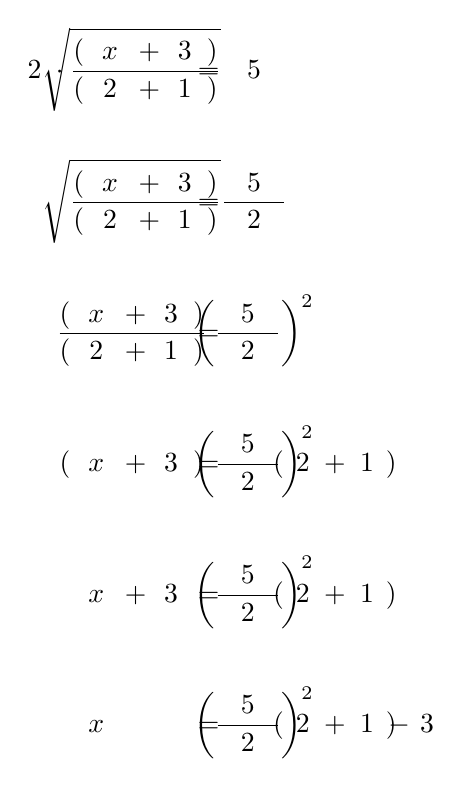
\begin{tikzpicture}[x=1em,y=-1em]
\node[anchor=base, inner sep=0pt] at (0.53,2.9) {$2$};
\node[anchor=base, inner sep=0pt] at (1.44,2.9) {$\cdot$};
\node[anchor=base, inner sep=0pt] at (4.04,2.9) {$\sqrt{\displaystyle\frac{\left(\pFourCell{1.88}{x}\pFourCell{0.96}{+}\pFourCell{1.6}{3}\right)}{\left(\pFourCell{1.88}{2}\pFourCell{0.96}{+}\pFourCell{1.6}{1}\right)}}$};
\node[anchor=base, inner sep=0pt] at (6.82,2.9) {$=$};
\node[anchor=base, inner sep=0pt] at (8.46,2.9) {$5$};
\node[anchor=base, inner sep=0pt] at (8.46,7.65) {$\displaystyle\frac{\pFourCell{2.16}{5}}{\pFourCell{2.16}{2}}$};
\node[anchor=base, inner sep=0pt] at (4.04,7.65) {$\sqrt{\displaystyle\frac{\left(\pFourCell{1.88}{x}\pFourCell{0.96}{+}\pFourCell{1.6}{3}\right)}{\left(\pFourCell{1.88}{2}\pFourCell{0.96}{+}\pFourCell{1.6}{1}\right)}}$};
\node[anchor=base, inner sep=0pt] at (6.82,7.65) {$=$};
\node[anchor=base, inner sep=0pt] at (4.04,12.385) {$\displaystyle\frac{\left(\pFourCell{1.88}{x}\pFourCell{0.96}{+}\pFourCell{1.6}{3}\right)}{\left(\pFourCell{1.88}{2}\pFourCell{0.96}{+}\pFourCell{1.6}{1}\right)}$};
\node[anchor=base, inner sep=0pt] at (6.82,12.385) {$=$};
\node[anchor=base, inner sep=0pt] at (8.46,12.385) {$\left(\displaystyle\frac{\pFourCell{2.16}{5}}{\pFourCell{2.16}{2}}\right)^{2}$};
\node[anchor=base, inner sep=0pt] at (4.04,17.105) {$\left(\pFourCell{1.88}{x}\pFourCell{0.96}{+}\pFourCell{1.6}{3}\right)$};
\node[anchor=base, inner sep=0pt] at (6.82,17.105) {$=$};
\node[anchor=base, inner sep=0pt] at (8.46,17.105) {$\left(\displaystyle\frac{\pFourCell{2.16}{5}}{\pFourCell{2.16}{2}}\right)^{2}$};
\node[anchor=base, inner sep=0pt] at (11.38,17.105) {$\left(\pFourCell{1.36}{2}\pFourCell{0.96}{+}\pFourCell{1.36}{1}\right)$};
\node[anchor=base, inner sep=0pt] at (2.76,21.825) {$x$};
\node[anchor=base, inner sep=0pt] at (4.18,21.825) {$+$};
\node[anchor=base, inner sep=0pt] at (5.46,21.825) {$3$};
\node[anchor=base, inner sep=0pt] at (6.82,21.825) {$=$};
\node[anchor=base, inner sep=0pt] at (8.46,21.825) {$\left(\displaystyle\frac{\pFourCell{2.16}{5}}{\pFourCell{2.16}{2}}\right)^{2}$};
\node[anchor=base, inner sep=0pt] at (11.38,21.825) {$\left(\pFourCell{1.36}{2}\pFourCell{0.96}{+}\pFourCell{1.36}{1}\right)$};
\node[anchor=base, inner sep=0pt] at (2.76,26.545) {$x$};
\node[anchor=base, inner sep=0pt] at (6.82,26.545) {$=$};
\node[anchor=base, inner sep=0pt] at (8.46,26.545) {$\left(\displaystyle\frac{\pFourCell{2.16}{5}}{\pFourCell{2.16}{2}}\right)^{2}$};
\node[anchor=base, inner sep=0pt] at (11.38,26.545) {$\left(\pFourCell{1.36}{2}\pFourCell{0.96}{+}\pFourCell{1.36}{1}\right)$};
\node[anchor=base, inner sep=0pt] at (13.7,26.545) {$-$};
\node[anchor=base, inner sep=0pt] at (14.71,26.545) {$3$};
\end{tikzpicture}
\end{center}

\newpage
\section*{Spaltentreue LaTeX-Ausgabe mit Spaltengrenzen}
\vspace{6mm}
\begin{center}
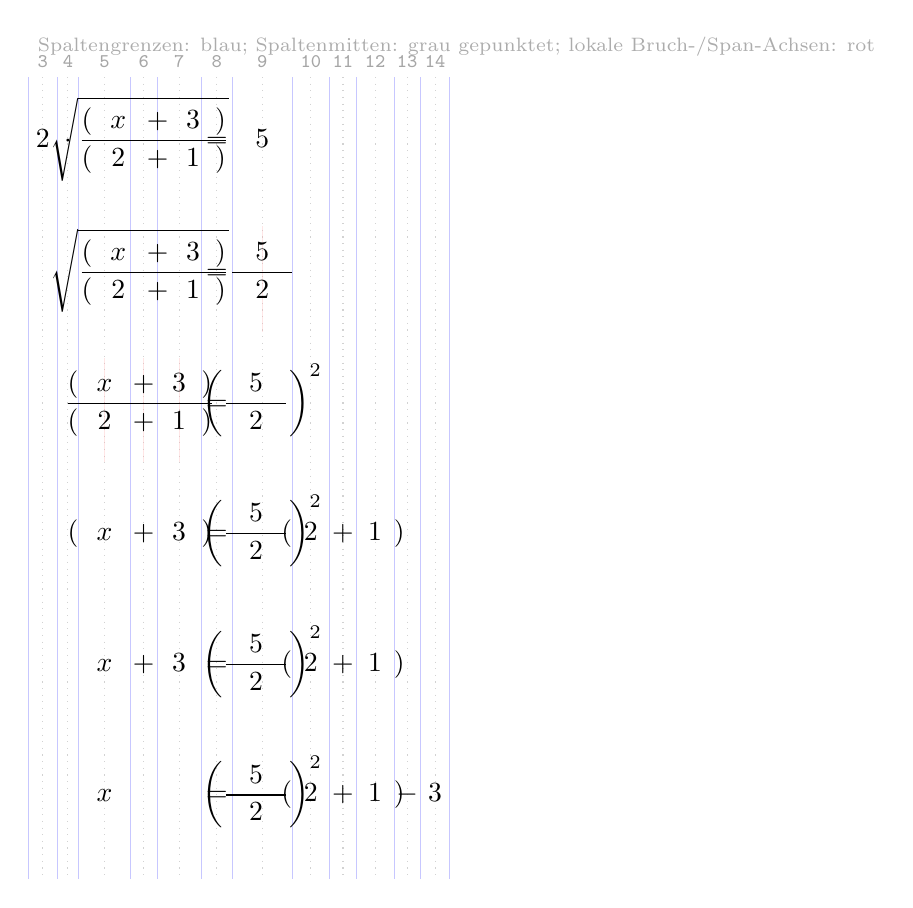
\begin{tikzpicture}[x=1em,y=-1em]
\node[font={\scriptsize}, text=gray!65, anchor=west] at (0,-0.75) {Spaltengrenzen: blau; Spaltenmitten: grau gepunktet; lokale Bruch-/Span-Achsen: rot};
\draw[blue!22, line width=0.28pt] (0,0.35) -- (0,29.33);
\draw[blue!22, line width=0.28pt] (1.06,0.35) -- (1.06,29.33);
\draw[blue!22, line width=0.28pt] (1.82,0.35) -- (1.82,29.33);
\draw[blue!22, line width=0.28pt] (3.7,0.35) -- (3.7,29.33);
\draw[blue!22, line width=0.28pt] (4.66,0.35) -- (4.66,29.33);
\draw[blue!22, line width=0.28pt] (6.26,0.35) -- (6.26,29.33);
\draw[blue!22, line width=0.28pt] (7.38,0.35) -- (7.38,29.33);
\draw[blue!22, line width=0.28pt] (9.54,0.35) -- (9.54,29.33);
\draw[blue!22, line width=0.28pt] (10.9,0.35) -- (10.9,29.33);
\draw[blue!22, line width=0.28pt] (11.86,0.35) -- (11.86,29.33);
\draw[blue!22, line width=0.28pt] (13.22,0.35) -- (13.22,29.33);
\draw[blue!22, line width=0.28pt] (14.18,0.35) -- (14.18,29.33);
\draw[blue!22, line width=0.28pt] (15.24,0.35) -- (15.24,29.33);
\draw[gray!35, dotted] (0.53,0.35) -- (0.53,29.33);
\node[font={\ttfamily\scriptsize}, text=gray!70, anchor=base] at (0.53,0) {3};
\draw[gray!35, dotted] (1.44,0.35) -- (1.44,29.33);
\node[font={\ttfamily\scriptsize}, text=gray!70, anchor=base] at (1.44,0) {4};
\draw[gray!35, dotted] (2.76,0.35) -- (2.76,29.33);
\node[font={\ttfamily\scriptsize}, text=gray!70, anchor=base] at (2.76,0) {5};
\draw[gray!35, dotted] (4.18,0.35) -- (4.18,29.33);
\node[font={\ttfamily\scriptsize}, text=gray!70, anchor=base] at (4.18,0) {6};
\draw[gray!35, dotted] (5.46,0.35) -- (5.46,29.33);
\node[font={\ttfamily\scriptsize}, text=gray!70, anchor=base] at (5.46,0) {7};
\draw[gray!35, dotted] (6.82,0.35) -- (6.82,29.33);
\node[font={\ttfamily\scriptsize}, text=gray!70, anchor=base] at (6.82,0) {8};
\draw[gray!35, dotted] (8.46,0.35) -- (8.46,29.33);
\node[font={\ttfamily\scriptsize}, text=gray!70, anchor=base] at (8.46,0) {9};
\draw[gray!35, dotted] (10.22,0.35) -- (10.22,29.33);
\node[font={\ttfamily\scriptsize}, text=gray!70, anchor=base] at (10.22,0) {10};
\draw[gray!35, dotted] (11.38,0.35) -- (11.38,29.33);
\node[font={\ttfamily\scriptsize}, text=gray!70, anchor=base] at (11.38,0) {11};
\draw[gray!35, dotted] (12.54,0.35) -- (12.54,29.33);
\node[font={\ttfamily\scriptsize}, text=gray!70, anchor=base] at (12.54,0) {12};
\draw[gray!35, dotted] (13.7,0.35) -- (13.7,29.33);
\node[font={\ttfamily\scriptsize}, text=gray!70, anchor=base] at (13.7,0) {13};
\draw[gray!35, dotted] (14.71,0.35) -- (14.71,29.33);
\node[font={\ttfamily\scriptsize}, text=gray!70, anchor=base] at (14.71,0) {14};
\node[anchor=base, inner sep=0pt] at (0.53,2.9) {$2$};
\node[anchor=base, inner sep=0pt] at (1.44,2.9) {$\cdot$};
\node[anchor=base, inner sep=0pt] at (4.04,2.9) {$\sqrt{\displaystyle\frac{\left(\pFourCell{1.88}{x}\pFourCell{0.96}{+}\pFourCell{1.6}{3}\right)}{\left(\pFourCell{1.88}{2}\pFourCell{0.96}{+}\pFourCell{1.6}{1}\right)}}$};
\node[anchor=base, inner sep=0pt] at (6.82,2.9) {$=$};
\node[anchor=base, inner sep=0pt] at (8.46,2.9) {$5$};
\draw[red!30, opacity=0.32, line width=0.35pt] (8.46,5.75) -- (8.46,9.55);
\node[anchor=base, inner sep=0pt] at (8.46,7.65) {$\displaystyle\frac{\pFourCell{2.16}{5}}{\pFourCell{2.16}{2}}$};
\node[anchor=base, inner sep=0pt] at (4.04,7.65) {$\sqrt{\displaystyle\frac{\left(\pFourCell{1.88}{x}\pFourCell{0.96}{+}\pFourCell{1.6}{3}\right)}{\left(\pFourCell{1.88}{2}\pFourCell{0.96}{+}\pFourCell{1.6}{1}\right)}}$};
\node[anchor=base, inner sep=0pt] at (6.82,7.65) {$=$};
\draw[red!30, opacity=0.32, line width=0.35pt] (2.76,10.5) -- (2.76,14.27);
\draw[red!30, opacity=0.32, line width=0.35pt] (4.18,10.5) -- (4.18,14.27);
\draw[red!30, opacity=0.32, line width=0.35pt] (5.46,10.5) -- (5.46,14.27);
\node[anchor=base, inner sep=0pt] at (4.04,12.385) {$\displaystyle\frac{\left(\pFourCell{1.88}{x}\pFourCell{0.96}{+}\pFourCell{1.6}{3}\right)}{\left(\pFourCell{1.88}{2}\pFourCell{0.96}{+}\pFourCell{1.6}{1}\right)}$};
\node[anchor=base, inner sep=0pt] at (6.82,12.385) {$=$};
\node[anchor=base, inner sep=0pt] at (8.46,12.385) {$\left(\displaystyle\frac{\pFourCell{2.16}{5}}{\pFourCell{2.16}{2}}\right)^{2}$};
\node[anchor=base, inner sep=0pt] at (4.04,17.105) {$\left(\pFourCell{1.88}{x}\pFourCell{0.96}{+}\pFourCell{1.6}{3}\right)$};
\node[anchor=base, inner sep=0pt] at (6.82,17.105) {$=$};
\node[anchor=base, inner sep=0pt] at (8.46,17.105) {$\left(\displaystyle\frac{\pFourCell{2.16}{5}}{\pFourCell{2.16}{2}}\right)^{2}$};
\node[anchor=base, inner sep=0pt] at (11.38,17.105) {$\left(\pFourCell{1.36}{2}\pFourCell{0.96}{+}\pFourCell{1.36}{1}\right)$};
\node[anchor=base, inner sep=0pt] at (2.76,21.825) {$x$};
\node[anchor=base, inner sep=0pt] at (4.18,21.825) {$+$};
\node[anchor=base, inner sep=0pt] at (5.46,21.825) {$3$};
\node[anchor=base, inner sep=0pt] at (6.82,21.825) {$=$};
\node[anchor=base, inner sep=0pt] at (8.46,21.825) {$\left(\displaystyle\frac{\pFourCell{2.16}{5}}{\pFourCell{2.16}{2}}\right)^{2}$};
\node[anchor=base, inner sep=0pt] at (11.38,21.825) {$\left(\pFourCell{1.36}{2}\pFourCell{0.96}{+}\pFourCell{1.36}{1}\right)$};
\node[anchor=base, inner sep=0pt] at (2.76,26.545) {$x$};
\node[anchor=base, inner sep=0pt] at (6.82,26.545) {$=$};
\node[anchor=base, inner sep=0pt] at (8.46,26.545) {$\left(\displaystyle\frac{\pFourCell{2.16}{5}}{\pFourCell{2.16}{2}}\right)^{2}$};
\node[anchor=base, inner sep=0pt] at (11.38,26.545) {$\left(\pFourCell{1.36}{2}\pFourCell{0.96}{+}\pFourCell{1.36}{1}\right)$};
\node[anchor=base, inner sep=0pt] at (13.7,26.545) {$-$};
\node[anchor=base, inner sep=0pt] at (14.71,26.545) {$3$};
\end{tikzpicture}
\end{center}
\end{document}
